\documentclass[11pt]{article}
\usepackage[a4paper,margin=1in]{geometry}
\usepackage[T1]{fontenc}
\usepackage{lmodern}
\usepackage{microtype}
\usepackage{amsmath,amssymb,amsthm}
\usepackage{booktabs,tabularx,array}
\usepackage{enumitem}
\usepackage{xcolor}
\usepackage{listings}
\usepackage{tikz}
\usetikzlibrary{positioning,arrows.meta,fit}
\usepackage[colorlinks=true,linkcolor=blue!50!black,urlcolor=blue!50!black]{hyperref}

\setlist{itemsep=2pt,topsep=4pt}
\lstset{basicstyle=\ttfamily\small,columns=fullflexible,keepspaces=true,
  frame=single,framerule=0.3pt,xleftmargin=4pt,xrightmargin=4pt,
  aboveskip=8pt,belowskip=8pt,showstringspaces=false}

\newcommand{\kw}[1]{\texttt{#1}}
\newcommand{\nil}{\kw{0}}
\newcommand{\tru}{\kw{true}}
\newcommand{\fls}{\kw{false}}
\newcommand{\bnot}{\mathord{\sim}}
\newcommand{\band}{\mathbin{\&\&}}
\newcommand{\bor}{\mathbin{||}}
\newcommand{\bxor}{\mathbin{\kw{xor}}}
\newcommand{\quo}[1]{@#1}
\newcommand{\drp}[1]{{*}#1}
\newcommand{\for}[3]{\kw{for}(#1 \leftarrow #2)\,#3}
\newcommand{\forp}[3]{\kw{for}(#1 \Leftarrow #2)\,#3}
\newcommand{\snd}[2]{#1!(#2)}
\newcommand{\cpar}{\mathbin{|}}
\newcommand{\scong}{\equiv}
\newcommand{\nameq}{\equiv_N}
\newcommand{\red}{\rightarrow}
\newcommand{\nf}[1]{\mathsf{nf}(#1)}
\newcommand{\sem}[1]{[\![#1]\!]}
\newcommand{\dec}[1]{\textbf{D#1}}
\newcommand{\conf}{\textsc{c}}
\newcommand{\prop}{\textsc{p}}

\theoremstyle{definition}
\newtheorem{obligation}{Obligation}
\newtheorem{definition}{Definition}
\theoremstyle{remark}
\newtheorem{remark}{Remark}

\title{A Hardware Rendering of the Rho Calculus with Boolean Arithmetic\\[4pt]
\large Design specification: source language, target machine, and verification guidance}
\author{F1R3FLY.io design note --- draft 0.3}
\date{13 November 2026}

\begin{document}
\maketitle

\begin{abstract}
\noindent
This note specifies a first hardware rendering of the rho calculus extended
with Boolean arithmetic. It fixes the source language (syntax, sorts,
structural congruence, matching modulo the Boolean laws, and reduction), the
canonical forms that make names comparable in constant time, a synchronous
tuple-space machine that realises the calculus on an FPGA and ports unchanged
to a CMOS ASIC flow, the division of the implementation between Bluespec and
Clash, and the obligations an implementation must discharge to count as
verified. All decisions in the register of Section~\ref{sec:decisions} are confirmed.
One semantic question remains open and is stated in Section~\ref{sec:open}.
Draft 0.3 folds in six corrections found by building and testing the
reference implementation; they are listed in Section~\ref{sec:changes}.
\end{abstract}

\tableofcontents

%======================================================================
\section{Purpose and scope}

The goal is a machine whose instruction set \emph{is} the calculus: the only
state change is the COMM rule, and every source of nondeterminism in the
calculus is a physical arbitration in the machine. The first target is an
FPGA, described in a high-level hardware language that emits Verilog. The
design is restricted to components expressible in synthesizable
Verilog or VHDL for CMOS; clockless and superconducting realisations are out
of scope, but the interfaces are kept latency-insensitive so that a later
self-timed version does not require a redesign.

In scope: the calculus of Section~\ref{sec:source}; a single-reducer machine
with a path to parallel reduction; a compiler from source text to a memory
image; a verification plan. Out of scope for this draft: cost accounting,
join patterns, \kw{where} clauses and grading, the combinator instruction
set, and multi-chip sharding. Hooks are left where these attach
(Sections~\ref{sec:arbiter} and~\ref{sec:staging}).

%======================================================================
\section{Decision register}\label{sec:decisions}

\noindent
\begin{tabularx}{\textwidth}{@{}l X c@{}}
\toprule
ID & Decision & Status\\
\midrule
\dec{1} & Boolean operands admit drops: $\drp{x}$ is a Boolean expression. & \conf\\
\dec{2} & The Boolean-algebra laws are part of structural congruence. & \conf\\
\dec{3} & Replication is derivable by the reflective encoding; a persistent
          receive is provided as sugar and implemented as a primitive. & \conf\\
\dec{4} & Ill-sorted terms are excluded by a basic spatial-behavioural type
          system, not by the machine. & \conf\\
\dec{5} & Distinct solutions of a Boolean pattern are distinct, observable
          races, on the same footing as COMM races. & \conf\\
\dec{6} & First target is an FPGA, via generated Verilog. & \conf\\
\dec{7} & A high-level functional hardware language is used in place of
          hand-written RTL. & \conf\\
\midrule
\dec{8} & Architecture: tuple-space machine (hash-consed term heap, channel
          store, matcher, arbiter). Static elaboration of the Boolean-typed
          fragment is a later optimisation. & \conf\\
\dec{9} & Tool split: Bluespec (BH syntax) for the rule-based reaction core;
          Clash for pure datapath functions; one Haskell reference library
          shared with the compiler. & \conf\\
\dec{10} & The compiler is trusted for sorts. The machine keeps a sticky
          \kw{FAULT\_SORT} flag whose unreachability is a proof obligation. The flag is a
          debugging aid: it does not detect every ill-sorted program. & \conf\\
\dec{11} & Variables are a separate syntactic category $V$, instantiated in
          the machine as de~Bruijn indices. Names remain quoted processes. & \conf\\
\dec{12} & Open Boolean code is canonicalised as a truth table over at most
          $K=6$ variables; larger supports are rejected at compile time. & \conf\\
\dec{13} & Boolean patterns (other than a bare variable) match closed Boolean
          values only. & \conf\\
\dec{14} & Fairness is possibilistic: every enabled redex has nonzero
          probability at every step. Uniformity over redexes is not required. & \conf\\
\dec{15} & Entropy is an LFSR behind an interface; every arbitration is
          written to a decision log that makes runs replayable. & \conf\\
\dec{16} & The machine is board-agnostic: no vendor primitives, inferred
          block RAM only, all sizes are parameters. & \conf\\
\bottomrule
\end{tabularx}

%======================================================================
\section{Source language}\label{sec:source}

\subsection{Syntax}

Let $V$ be a countable set of variables, ranged over by $v,w$. Processes
$P,Q$, Boolean expressions $B$, names $x,y$, patterns $p$ and deep patterns
$d$ are given by
\[
\begin{array}{rcl}
P,Q &::=& \nil \;\mid\; B \;\mid\; \for{p}{x}{P} \;\mid\; \forp{p}{x}{P}
          \;\mid\; \snd{x}{Q} \;\mid\; P \cpar Q \;\mid\; \drp{x}\\[2pt]
B &::=& \tru \;\mid\; \fls \;\mid\; \drp{x} \;\mid\; \bnot B \;\mid\; B \band B
          \;\mid\; B \bor B \;\mid\; B \bxor B\\[2pt]
x,y &::=& \quo{P} \;\mid\; v\\[2pt]
p &::=& v \;\mid\; \quo{d}\\[2pt]
d &::=& \nil \;\mid\; \tru \;\mid\; \fls \;\mid\; v \;\mid\; \snd{p}{d}
          \;\mid\; \for{v}{p}{d}
          \;\mid\; \bnot d \;\mid\; d \band d \;\mid\; d \bor d \;\mid\; d \bxor d
\end{array}
\]
Relative to the grammar that opened the session, \dec{1} adds $\drp{x}$ to
$B$, \dec{3} adds the persistent receive $\forp{p}{x}{P}$, and \dec{11}
separates variables from names. Quotation is written $\quo{P}$ and
dereference $\drp{x}$ throughout. The production $\drp{x}$ is shared by $P$
and $B$; which reading applies is settled by sorts.

A receive binds the variables of its pattern in its body. Every variable
denotes a \emph{name}. A variable in a deep-pattern position denotes the name
of the matched subprocess, so matching $\quo{(v \band w)}$ binds $v$ and $w$
to names of Booleans, and the body uses them as $\drp{v}$ and $\drp{w}$.
A program is a closed process.

\subsection{Sorts}\label{sec:sorts}

There are two sorts of process, $\mathsf{Bool} \subseteq \mathsf{Proc}$, and
correspondingly two sorts of variable: \emph{Boolean-sorted} variables, which
only ever denote $\quo{\tru}$ or $\quo{\fls}$, and \emph{structural}
variables, which may denote any name. A term is well sorted when every
operand of a Boolean operator is of sort $\mathsf{Bool}$; in particular
$\drp{v}$ as an operand requires $v$ to be Boolean-sorted, and a
Boolean-sorted variable requires every message that can reach its receive to
quote a Boolean.

The last condition is a property of channels, and is discharged by the
spatial-behavioural type system (\dec{4}), which assigns a carried sort to
each namespace. This note treats that system as a black box with the
following interface.
\begin{itemize}
\item \textbf{Input.} A closed process.
\item \textbf{Output.} Either a rejection, or a sort for every pattern
variable, such that reduction preserves well-sortedness.
\end{itemize}
The reflective encoding of replication sends a quoted process on a channel
that the process itself mentions, so the system needs a recursive formula to
type it. Giving the persistent receive its own typing rule avoids that for
programs that use only the sugar.

\subsection{Structural congruence}\label{sec:cong}

Structural congruence $\scong$ is the least congruence on processes
containing:
\begin{enumerate}
\item alpha-equivalence of bound variables;
\item $(P \cpar Q) \cpar R \scong P \cpar (Q \cpar R)$,\quad
      $P \cpar Q \scong Q \cpar P$,\quad $P \cpar \nil \scong P$;
\item the laws of Boolean algebra on $B$, with $\bxor$ defined by
      $B_1 \bxor B_2 \scong (B_1 \band \bnot B_2) \bor (\bnot B_1 \band B_2)$;
\item $\drp{\quo{P}} \scong P$.
\end{enumerate}
Name equivalence $\nameq$ is the least equivalence with
$\quo{P} \nameq \quo{Q}$ whenever $P \scong Q$, and $\quo{\drp{x}} \nameq x$.
Law~4 is adopted as a convention; in the original presentation the same
effect arises only through substitution.

By \dec{2} every closed Boolean expression is congruent to exactly one of
\tru\ or \fls, so there are exactly two closed Boolean names up to $\nameq$.
The requirement that substituting a Boolean name into $\drp{y}$ yields the
\emph{evaluation} of the Boolean is therefore a consequence of law~3 and not
a separate rule: evaluation is normalisation.

\subsection{Matching}\label{sec:matching}

A substitution $\sigma$ maps variables to closed names and respects sorts.
\begin{definition}[Match set]
For a pattern $p$ and a closed name $n$,
\[
\mathsf{match}(p,n) \;=\; \{\, \sigma \mid \mathrm{dom}(\sigma)=\mathrm{vars}(p),\;
p\sigma \nameq n \,\}\big/{\nameq}
\]
where substitutions are identified when they agree pointwise up to $\nameq$.
\end{definition}
Matching is \emph{modulo} $\scong$. For structural patterns this is ordinary
tree matching on normal forms, and the match set has at most one element. For
Boolean patterns it is equation solving: $\mathsf{match}(\quo{(v \band w)},
\quo{\fls})$ has three elements and $\mathsf{match}(\quo{(v \band w)},
\quo{\tru})$ has one. Because Boolean-sorted variables range over two classes,
a pattern with $k$ Boolean variables has at most $2^k$ solutions.

\paragraph{Restrictions.}
\begin{itemize}
\item (\dec{13}) A Boolean pattern built with an operator matches only a
closed Boolean value. Matching an operator pattern against open Boolean code
under a binder would be unification of Boolean functions and is excluded. A Boolean
leaf, a constant leaf included, that meets a name not quoting a Boolean is a
sort fault and not a failed match; so the pattern $\quo{\tru}$ cannot be used
to test whether a message is a Boolean.
\item A pattern variable is a \emph{mask variable} when it occurs under a
Boolean operator in the pattern; every occurrence of it is then a Boolean
leaf. Any other variable is bound structurally, whatever its sort, and its
sort is checked where the body uses it. A pattern has at most $K$ mask
variables (\dec{12}).
\item Deep patterns contain no parallel composition, as in the given
grammar, so no matching modulo associativity and commutativity is needed.
\item The receive pattern $\for{v}{p}{d}$, which matches under a binder, is
deferred; see Section~\ref{sec:open}.
\end{itemize}

\subsection{Reduction}\label{sec:reduction}

\[
\frac{x \nameq y \qquad \sigma \in \mathsf{match}(p,\quo{Q})}
     {\for{p}{x}{P} \cpar \snd{y}{Q} \;\red\; P\sigma}\;\textsc{(comm)}
\]
\[
\frac{x \nameq y \qquad \sigma \in \mathsf{match}(p,\quo{Q})}
     {\forp{p}{x}{P} \cpar \snd{y}{Q} \;\red\; P\sigma \cpar \forp{p}{x}{P}}\;\textsc{(comm!)}
\]
\[
\frac{P \red P'}{P \cpar Q \red P' \cpar Q}\;\textsc{(par)}
\qquad
\frac{P \scong P' \quad P' \red Q' \quad Q' \scong Q}{P \red Q}\;\textsc{(equiv)}
\]
There is no reduction under a receive or under a quote. Substitution
$P\sigma$ replaces free variables by names and does not descend into closed
quoted terms, which have no free variables.

A \emph{redex} of a process is a triple (send, receive, solution). By \dec{5}
two redexes that differ only in the solution are different transitions. A
send whose channel has a receive but whose payload admits no solution is not
a redex and stays in place.

\subsection{Replication}

With $D(x) = \for{v}{x}{(\snd{x}{\drp{v}} \cpar \drp{v})}$, replication of
$P$ on a name $x$ not otherwise used is
$\snd{x}{D(x) \cpar P} \cpar D(x)$. The machine must run this term correctly
without special support, which requires a general drop of quoted code.
The persistent receive is the efficient form. Its specification is the
encoding:
\begin{obligation}\label{ob:repl}
For all $p$, $x$, $P$, the process $\forp{p}{x}{P}$ is weakly bisimilar to
its reflective encoding, under context-labelled transitions.
\end{obligation}

%======================================================================
\section{Canonical forms}\label{sec:canon}

The machine compares names by comparing machine words. That is sound only if
every term is stored in a normal form that is unique up to $\scong$. The
normal form $\nf{P}$ is defined bottom-up.

\begin{description}
\item[Variables.] Bound variables are replaced by de~Bruijn indices: an
occurrence is the number of variable binders between it and its own binder,
counting each variable of a multi-variable pattern in left-to-right order of
first occurrence. Closed subterms therefore have a representation that does
not depend on their context, which is what permits sharing.
This indexes $V$ only; names are still quoted processes (\dec{11}).

\item[Quote and drop.] $\drp{\quo{P}}$ is replaced by $\nf{P}$, and
$\quo{\drp{x}}$ by $x$.

\item[Booleans.] A Boolean expression whose operands are all closed is
replaced by its value. Otherwise let $v_0 < \dots < v_{k-1}$ be the variables
it \emph{depends on} (its support), ordered by index. The normal form is the
pair of the support and the truth table $T \in \{0,1\}^{2^k}$, where bit
$r = \sum_i b_i 2^i$ of $T$ is the value of the expression at
$v_i \mapsto b_i$. Variables on which the function does not depend are
removed. A function that is the identity on a single variable $v$ is stored
as $\drp{v}$. If $k > K$ the program is rejected (\dec{12}).

\item[Parallel composition.] Compositions are flattened, $\nil$ units are
removed, and the components are sorted into ascending order of their machine
words. Since each component is itself canonical and hash-consed
(Section~\ref{sec:heap}), word order is a total order on components up to
$\scong$. Duplicates are kept: composition is a multiset.

\item[Other constructors.] Sends, receives and persistent receives are
normalised componentwise. Patterns are normalised by the compiler into
pattern programs (Section~\ref{sec:compiler}); two receives are congruent
only if their pattern programs are identical.
\end{description}

\begin{obligation}[Canonicity]\label{ob:canon}
For all well-sorted $P$, $Q$ within the size bounds:
$\nf{P} = \nf{Q}$ if and only if $P \scong Q$.
\end{obligation}

\begin{remark}
The truth table over a minimal, ordered support is a canonical form for
Boolean functions, so the Boolean part of Obligation~\ref{ob:canon} is
immediate. The same 64-bit word serves three purposes: it is the normal form,
it evaluates the function forwards (index it by the argument values), and it
solves patterns backwards (Section~\ref{sec:matcher}).
\end{remark}

%======================================================================
\section{Target machine}\label{sec:target}

\subsection{Overview}

\begin{figure}[h]
\centering
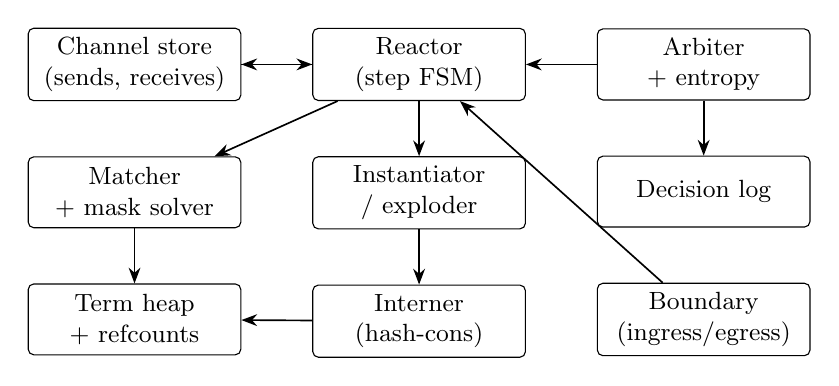
\begin{tikzpicture}[
  blk/.style={draw,rounded corners=2pt,minimum width=27mm,minimum height=9mm,
              align=center,font=\small},
  arr/.style={-{Stealth[length=2mm]},semithick},
  node distance=7mm and 9mm]
\node[blk] (store) {Channel store\\(sends, receives)};
\node[blk,right=of store] (react) {Reactor\\(step FSM)};
\node[blk,right=of react] (arb) {Arbiter\\+ entropy};
\node[blk,below=of store] (match) {Matcher\\+ mask solver};
\node[blk,below=of react] (inst) {Instantiator\\/ exploder};
\node[blk,below=of arb] (log) {Decision log};
\node[blk,below=of match] (heap) {Term heap\\+ refcounts};
\node[blk,below=of inst] (intern) {Interner\\(hash-cons)};
\node[blk,below=of log] (io) {Boundary\\(ingress/egress)};
\draw[arr] (store) -- (react);
\draw[arr] (react) -- (store);
\draw[arr] (arb) -- (react);
\draw[arr] (react) -- (match);
\draw[arr] (react) -- (inst);
\draw[arr] (arb) -- (log);
\draw[arr] (match) -- (heap);
\draw[arr] (inst) -- (intern);
\draw[arr] (intern) -- (heap);
\draw[arr] (io) -- (react);
\end{tikzpicture}
\caption{Blocks of the machine. Arrows show the direction of requests.}
\end{figure}

The machine holds the top level of the running process as a \emph{soup}: a
table of sends and a table of receives. Everything quoted lives in a
hash-consed heap of canonical terms. One \emph{step} selects a redex,
removes its send (and its receive, unless persistent), and adds the
components of the instantiated continuation to the soup. A step takes many
clock cycles; the calculus sees only step boundaries.

\subsection{Words and nodes}\label{sec:words}

All widths are parameters; the reference values are for a 32-bit word with a
28-bit heap address.

\medskip\noindent
\begin{tabularx}{\textwidth}{@{}l l X@{}}
\toprule
Word & Tag & Meaning\\
\midrule
Process word & \kw{ZERO} & the process $\nil$\\
             & \kw{BOOL} $b$ & the Boolean value $b$\\
             & \kw{PTR} $a$ & the process stored at heap address $a$\\
\addlinespace
Name word & \kw{QZERO} & the name $\quo{\nil}$\\
          & \kw{QBOOL} $b$ & the name $\quo{b}$\\
          & \kw{QPTR} $a$ & the name $\quo{}$(node at $a$)\\
          & \kw{VAR} $i$ & the variable with de~Bruijn index $i$ (code only)\\
\bottomrule
\end{tabularx}

\medskip\noindent
Closed Boolean names are immediates and never touch the heap.

\medskip\noindent
\begin{tabularx}{\textwidth}{@{}l X@{}}
\toprule
Node kind & Fields\\
\midrule
\kw{PAR}   & head: process word; tail: process word (a \kw{PAR} or the last component)\\
\kw{SEND}  & chan: name word; payload: process word\\
\kw{RECV}  & chan: name word; pat: pattern-program address; body: process
             word; nvars; persistent bit\\
\kw{DROP}  & name: name word (always a \kw{VAR}, by normalisation)\\
\kw{BFN}   & arity $k \le K$; support: $k$ variable indices, ascending;
             table: $2^K$ bits\\
\bottomrule
\end{tabularx}

\medskip\noindent
Every node carries a header with its kind, a \emph{free-variable depth}, and
a \emph{sort} bit (the node is of sort $\mathsf{Bool}$). The depth of a node
is the least $k$ such that every free variable index in it is below $k$; a
node is \emph{closed} when its depth is zero. Both fields are computed at
interning time from the children: a variable $i$ has depth $i+1$; a receive
with $n$ pattern variables has depth $\max(d_{\mathit{chan}},\, d_{\mathit{body}}-n,\, 0)$;
every other node takes the maximum over its fields. A single closed bit would
not do: whether a receive is closed depends on whether its body's free
variables are all bound by its own pattern, which a bit on the body cannot
tell. The exact packing into block-RAM words is left to the
implementation; it must be fixed in one shared definition used by the
compiler, the reference model and the hardware.

\subsection{Heap, interner and reference counts}\label{sec:heap}

\begin{itemize}
\item \textbf{Heap.} An array of nodes in block RAM with a free list.
\item \textbf{Interner.} \kw{intern(node)} returns the address of the unique
stored node equal to its argument, allocating if there is none. It is a
multi-cycle operation: hash the node contents, probe a hash table in block
RAM, and confirm any hit by a full field comparison. Equality is exact; the
hash only selects the bucket, so there is no collision risk.
\item \textbf{Normalising constructors.} The interner is the only way to
create a node, and each constructor normalises: \kw{PAR} performs the sorted
insertion of Section~\ref{sec:canon}; \kw{BFN} minimises the support and
collapses constants and projections; \kw{DROP} of a closed name returns the
named process.
\item \textbf{Reference counts.} Terms are acyclic, so reference counting
reclaims everything. A count is held per node in a separate RAM.
Decrements that reach zero push the node on a deferred-free stack that is
drained when the reactor is idle, which bounds the work per cycle.
\end{itemize}

\subsection{Channel store}

Two tables, each with a valid bit per entry.
\begin{itemize}
\item \textbf{Send table} $S[0..N_S)$: channel (closed name word), payload
(closed process word).
\item \textbf{Receive table} $R[0..N_R)$: channel (closed name word),
pattern-program address, body (process word, code), environment address,
persistent bit.
\end{itemize}
A receive in the soup is a \emph{closure}: its body is shared code and its
free variables are supplied by an environment, a heap-allocated vector of
closed name words. Anything that becomes a \emph{name} is fully instantiated
instead (Section~\ref{sec:inst}), since names must be canonical to be
compared.

Lookup by channel is a comparison of one name word against all entries of the
other table. In the first stages this is a register array with $N_R$
comparators. It is replaced by a block-RAM hash table keyed on the channel
word when table sizes outgrow that.

Top-level processes that are Boolean values are inert. They are counted in a
two-counter \emph{residue} register so that they remain observable.

\subsection{Matcher and mask solver}\label{sec:matcher}

The compiler turns each pattern into a \emph{pattern program}, a short
sequence of operations executed against a name word with an explicit cursor
stack.

\medskip\noindent
\begin{tabularx}{\textwidth}{@{}l X@{}}
\toprule
Operation & Effect\\
\midrule
\kw{NBIND}       & bind the current name word to the next structural variable\\
\kw{NEQ} $i$     & fail unless the current name word equals structural variable $i$\\
\kw{QZERO}       & fail unless the current name word is \kw{QZERO}\\
\kw{QSEND}       & fail unless the current name quotes a \kw{SEND}; push the
                   quoted payload, then continue with the channel\\
\kw{BLEAF} $T$   & raise \kw{FAULT\_SORT} unless the current name word is \kw{QBOOL} $b$;
                   set $\mathit{mask} \leftarrow \mathit{mask} \wedge
                   (b \mathrel{?} T : \neg T)$\\
\kw{END}         & succeed if the cursor stack is empty\\
\bottomrule
\end{tabularx}

\medskip\noindent
All Boolean leaves of one pattern are expressed by the compiler over a single
ordered space of that pattern's mask variables, so their masks conjoin
directly. The mask starts as all ones. The result of a successful run is the
vector of structural bindings and the mask.

\begin{itemize}
\item The mask is the solution set: bit $r$ is set exactly when the
assignment $v_i \mapsto$ bit $i$ of $r$ solves every Boolean leaf.
\item The pair is a redex if and only if the run succeeds and the mask is
nonzero.
\item The solver returns $\mathit{count} = \mathrm{popcount}(\mathit{mask})$
and, given $u < \mathit{count}$ from the arbiter, the index $r$ of the
$u$-th set bit. An occurrence of a mask variable outside any operator is a leaf whose table
is a projection, and a non-linear Boolean pattern such as
$v \band \bnot v$ needs no special case. A variable that occurs under no
operator is not a mask variable and is bound by \kw{NBIND}, as in the AND gate
of Appendix~\ref{sec:examples}.
\end{itemize}
The pure parts (mask update, popcount, select) are combinational functions
and are among the Clash components of Section~\ref{sec:tooling}.

\subsection{Arbiter and entropy}\label{sec:arbiter}

All nondeterminism of the calculus passes through one module with one
operation: \kw{choose(n)} returns $u \in [0,n)$ for $n \ge 1$. It is used
three times per step: to pick a send, to pick a receive among those on the
same channel, and to pick a solution row.

\begin{itemize}
\item \textbf{No pruning.} For every $n$ and every $u<n$ there must be an
entropy value for which \kw{choose(n)} returns $u$. A priority encoder is
forbidden: it would make the machine a refinement of the calculus and not
bisimilar to it.
\item \textbf{Entropy.} The reference source is a 32-bit maximal-length
Galois LFSR with taps 32, 22, 2 and 1. A choice among $n$ takes a 32-bit
sample $w$ and returns $\lfloor w\,n / 2^{32} \rfloor$. The reference model
advances the register 32 positions per choice, so that successive choices use
disjoint bits. Hardware with a free-running register need not match this,
because runs are compared through the decision log and not through seeds. A
hardware random source may replace the register behind the same interface.
\item \textbf{Fairness.} Only possibilistic fairness is required (\dec{14}).
The three-stage choice does not induce the uniform distribution over
redexes. When grading is added, each stage takes a weight vector in place of
a count, and weighting a pair by its solution count makes the composite
uniform; the \kw{choose} interface is defined so that this is a change of
argument type only.
\item \textbf{Replay.} In replay mode the arbiter ignores entropy and takes
its results from the decision log.
\end{itemize}

\subsection{The step}\label{sec:step}

The reactor is a state machine. States in which the abstraction function of
Section~\ref{sec:verification} is defined are called \emph{boundaries}.

\begin{enumerate}
\item \textbf{IDLE} (boundary). Drain deferred frees and accept ingress
(Section~\ref{sec:boundary}). If the send table is empty, stay.
\item \textbf{PICK-SEND.} Choose a valid send $s$ uniformly. Clear the
per-scan \emph{tried} vectors.
\item \textbf{PICK-RECV.} Compare the channel of $s$ with every valid
receive not yet tried for $s$. If none matches, mark $s$ tried; if all sends
are tried, the soup is \emph{quiescent}: set the status bit and return to
IDLE; otherwise choose another untried send. If some match, choose one, $r$.
\item \textbf{MATCH.} Run the pattern program of $r$ on the quoted payload
of $s$. On failure or zero mask, mark $r$ tried for $s$ and return to
PICK-RECV.
\item \textbf{COMMIT.} Choose a solution row. Write the log record. Remove
$s$; remove $r$ unless persistent. Build the new environment: the
environment of $r$ extended by the structural bindings and, for each mask
variable, the \kw{QBOOL} of its bit in the row. Variables enter in a fixed
order: structural variables in order of first occurrence in the pattern
program, then mask variables in order of mask position, so that the last
mask variable is the most recently bound.
\item \textbf{EXPLODE.} Walk the body of $r$ with the new environment and
add its top-level components to the soup (below).
\item Return to IDLE.
\end{enumerate}
A failed scan changes no state, so the scan terminates after at most
$N_S \times N_R$ matcher runs, and quiescence is detected exactly.

\paragraph{Explode.} A work stack holds (process word, environment) pairs.
\begin{itemize}
\item \kw{PAR}: push head and tail.
\item \kw{SEND}: resolve the channel through the environment, instantiate
the payload (Section~\ref{sec:inst}), insert into $S$, or emit on egress.
\item \kw{RECV}: resolve the channel, insert a closure into $R$.
\item \kw{DROP} of variable $i$: look up the name. \kw{QZERO}: nothing.
\kw{QBOOL}: increment the residue. \kw{QPTR}: push the named process with an
empty environment. This is the general drop that the replication encoding
needs; because the quoted term is closed and shared, it costs no copying.
\item \kw{BFN}: evaluate the table at the environment values; increment the
residue.
\item \kw{BOOL}: increment the residue. \kw{ZERO}: nothing.
\end{itemize}

\subsection{Instantiation}\label{sec:inst}

\kw{inst(code, env)} returns the canonical closed term obtained by
substituting the environment into the code. It is a post-order walk with an
explicit stack that rebuilds nodes through the interner, tracking the number
$k$ of binders passed.
\begin{itemize}
\item A subterm whose free-variable depth is at most $k$ is returned
unchanged: it mentions no variable beyond the binders already passed. This is
the common case and makes instantiation proportional to the open part of the
code only.
\item \kw{VAR} $i$ with $i<k$ is local and unchanged; with $i \ge k$ it is
replaced by environment entry $i-k$, where entries are numbered from the most
recently bound. Environment entries are closed, so no index shifting is needed.
\item A \kw{BFN} whose support becomes partly known is cofactored on the
known variables and re-normalised; when fully known it becomes a \kw{BOOL}.
\end{itemize}

\subsection{Boundary}\label{sec:boundary}

The environment is modelled as processes on designated channels, fixed in the
image.
\begin{itemize}
\item \textbf{Ingress.} Each input port is a channel. A valid/ready
interface inserts a send on that channel, accepted only in IDLE. In the first
stages the payload is restricted to immediates, and the sort tag is checked
against the port's declared sort; a mismatch is dropped and counted.
\item \textbf{Egress.} Each output port is a channel on which the environment
is the only receiver. A send on such a channel is emitted on the port's
valid/ready interface and is not stored.
\end{itemize}

\subsection{Decision log and faults}\label{sec:log}

One record per step: step number, send slot, receive slot, solution row. A
separate \emph{insert} stream reports every entry added to $S$ or $R$ with
its slot, and a \emph{residue} stream reports residue increments. Together
these let an external checker reconstruct the soup without reading the
machine's internals.

Faults are sticky status bits that halt the reactor at the next boundary.

\medskip\noindent
\begin{tabularx}{\textwidth}{@{}l X@{}}
\toprule
Fault & Raised when\\
\midrule
\kw{FAULT\_SORT} & a Boolean operand or Boolean leaf meets a non-Boolean
                   name. Unreachable for well-sorted programs (\dec{10}).\\
\kw{FAULT\_HEAP} & the heap, hash table or environment space is exhausted\\
\kw{FAULT\_STORE} & a send or receive table is full\\
\kw{FAULT\_STACK} & a work stack overflows\\
\bottomrule
\end{tabularx}

\medskip\noindent
Resource faults are the only way the machine departs from the calculus, and
they are detected, never silent.

\begin{remark}[The sort flag is not a sort check]
A Boolean law can erase an ill-sorted operand before anything inspects it:
$\drp{v} \bxor \drp{v}$ normalises to \fls\ and $\drp{v} \band \tru$ to
$\drp{v}$, whatever $v$ is later bound to. \kw{FAULT\_SORT} therefore fires
only for operands that survive normalisation. Its never firing does not show
that a program is well sorted, and Obligation~\ref{ob:sort} cannot be turned
round. The sort checker carries the whole obligation.
\end{remark}

\subsection{Parameters}

\noindent
\begin{tabularx}{\textwidth}{@{}l l X@{}}
\toprule
Parameter & Stage~1 value & Meaning\\
\midrule
$K$ & 6 & maximum Boolean support and pattern mask variables\\
$N_S$, $N_R$ & 64, 64 & send and receive table sizes\\
$A$ & 28 (later) & heap address width; stage~1 has no dynamic heap\\
$E$ & 16 & maximum environment length\\
$D$ & 32 & work-stack depth\\
LFSR width & 32 & entropy state\\
\bottomrule
\end{tabularx}

%======================================================================
\section{Tooling and code organisation}\label{sec:tooling}

\subsection{Division of labour (\dec{9})}

\begin{description}
\item[Reference library (plain Haskell).] Abstract syntax, normal forms,
match sets, the one-step relation returning \emph{all} redexes, and the node
packing. This is the executable semantics. The compiler and the checker are
built on it.
\item[Clash.] The pure, combinational datapath: truth-table operations
(negate, combine over merged supports, minimise support, cofactor), mask
update, popcount and select, the node hash, node encode and decode. These are
ordinary Haskell functions over sized types, and they are written once and
imported both by the reference library and by the Clash top entities, so
there is a single source for each.
\item[Bluespec (BH).] Everything with state and scheduling: heap, interner,
store, matcher sequencer, instantiator, arbiter, reactor, log, boundary. The
calculus is a rewrite system and Bluespec's guarded atomic rules express each
transition of Section~\ref{sec:step} directly.
\end{description}
Clash-generated Verilog modules are imported into Bluespec as combinational
foreign modules. If the two-tool flow proves costly, the fallback is Clash
alone, with the reactor written as an explicit Mealy machine; nothing in
this specification depends on Bluespec.

\subsection{Rules for the Bluespec code}

\begin{enumerate}
\item Every semantically visible choice goes through the arbiter module.
The Bluespec scheduler resolves rule conflicts by a fixed urgency order,
which is a priority encoder; it must never be the thing that decides which
redex fires.
\item Any urgency annotation must carry a comment stating why the conflict
it resolves is invisible at boundaries.
\item Each rule that changes the store or the heap states, as an assertion,
the invariants of Section~\ref{sec:invariants} it relies on.
\item No vendor primitives. Memories are inferred. One clock, synchronous
reset.
\end{enumerate}

\subsection{Suggested module list}

\noindent
\begin{tabularx}{\textwidth}{@{}l l X@{}}
\toprule
Module & Tool & Responsibility\\
\midrule
\kw{TruthTable}   & Clash & table algebra and normalisation\\
\kw{MaskSolve}    & Clash & mask, popcount, select\\
\kw{NodeCodec}    & Clash & packing, hash, free-variable depth and sort bit\\
\kw{mkHeap}       & BH & node RAM, free list, reference counts\\
\kw{mkInterner}   & BH & hash-cons table, normalising constructors\\
\kw{mkStore}      & BH & send and receive tables, channel lookup\\
\kw{mkMatcher}    & BH & pattern-program sequencer\\
\kw{mkInst}       & BH & instantiate and explode walkers\\
\kw{mkArbiter}    & BH & \kw{choose}, LFSR, replay input\\
\kw{mkReactor}    & BH & the step state machine\\
\kw{mkLog}        & BH & decision, insert and residue streams\\
\kw{mkBoundary}   & BH & ingress and egress ports\\
\bottomrule
\end{tabularx}

\subsection{Flow}

Source text $\to$ compiler $\to$ memory image. Bluespec and Clash $\to$
Verilog $\to$ simulation (Verilator) and synthesis (vendor or open flow).
The same Verilog is the input to bounded formal checks.

%======================================================================
\section{Compiler and image}\label{sec:compiler}

The compiler is software and is in the trusted base for sorts only
(\dec{10}); every other property of its output is checked dynamically by the
verification harness.

\begin{enumerate}
\item Parse; resolve variables to de~Bruijn indices.
\item Run the sort checker; record each pattern variable's sort.
\item Normalise (Section~\ref{sec:canon}); reject Boolean supports above $K$.
\item Compile patterns to pattern programs. Assign mask variables their
positions in the pattern's mask space and extend each leaf table to that
space.
\item Intern all code into a heap image using the same interner algorithm
as the hardware, so that addresses in the image are canonical.
\item Explode the top-level process into initial send and receive tables.
\item Emit block-RAM initialisation files for the heap, hash table, reference
counts, pattern store and the two tables, plus a symbol file mapping source
names to name words for the test harness.
\end{enumerate}

%======================================================================
\section{Verification}\label{sec:verification}

\subsection{What ``verified'' means}

Let $\alpha$ map a machine state at a boundary to a process:
\[
\alpha(s) \;=\; \prod_{i \in S} \snd{c_i}{q_i} \;\cpar\;
                \prod_{j \in R} \mathsf{inst}(\mathit{recv}_j,\mathit{env}_j)
                \;\cpar\; \tru^{\,t} \cpar \fls^{\,f}
\]
where $(t,f)$ is the residue and all terms are read back from the heap.

\begin{obligation}[Soundness]\label{ob:sound}
If the machine goes from boundary $s$ to the next boundary $s'$ by a step,
then $\alpha(s) \red \alpha(s')$.
\end{obligation}
\begin{obligation}[No pruning]\label{ob:complete}
If $\alpha(s) \red Q$ and no resource fault occurs, there is a sequence of
arbiter results for which the next boundary $s'$ satisfies
$\alpha(s') \scong Q$.
\end{obligation}
\begin{obligation}[Quiescence]\label{ob:quiet}
The quiescent bit is set at a boundary if and only if $\alpha(s)$ has no
redex.
\end{obligation}
\begin{obligation}[Replay]\label{ob:replay}
Two runs from the same image with the same ingress sequence and the same
decision log pass through identical boundary states.
\end{obligation}
\begin{obligation}[Sort safety]\label{ob:sort}
For a well-sorted image, \kw{FAULT\_SORT} is unreachable.
\end{obligation}
Obligations \ref{ob:sound} and \ref{ob:complete} together say that $\alpha$
is a bisimulation between the fault-free machine, observed at boundaries, and
the calculus. Obligations \ref{ob:repl} and \ref{ob:canon} are the supporting
facts about the language itself.

\subsection{Layers of evidence}

\noindent
\begin{tabularx}{\textwidth}{@{}l X X@{}}
\toprule
Layer & Method & Discharges\\
\midrule
V1 & Property tests of the reference normaliser against a brute-force
     decision of $\scong$ on small terms; exhaustive for Boolean code with
     $k \le 3$ & Ob.~\ref{ob:canon} (reference)\\
V2 & The Clash functions are the reference functions: test in GHC, then
     check generated Verilog against them by random co-simulation
     & datapath correctness\\
V3 & Interner test: intern random raw terms through the machine's normalising
     constructors alone; addresses equal iff reference normal forms equal,
     and readback equals the reference normal form & Ob.~\ref{ob:canon} (hardware)\\
V4 & Step-refinement checker (below) on random and directed programs
     & Ob.~\ref{ob:sound}, \ref{ob:quiet}\\
V5 & Formal cover on the arbiter: for every $n \le 64$ and $u<n$ a
     witness entropy value exists & Ob.~\ref{ob:complete} (arbiter)\\
V6 & Redex coverage: on small programs, every reference redex at every
     visited state is taken under some seed & Ob.~\ref{ob:complete} (system)\\
V7 & Replay test: record, replay, compare boundary traces
     & Ob.~\ref{ob:replay}\\
V8 & Assertions for the invariants below, in simulation and bounded
     model checking & supports all\\
V9 & Bounded bisimulation check, in the reference, of persistent receive
     against the encoding; paper proof to follow & Ob.~\ref{ob:repl}\\
V10 & Instantiation commutes with normalisation, in the reference and in the
     machine, against textbook substitution on raw terms
     & Ob.~\ref{ob:sound} (instantiation)\\
V11 & Mutation: each of a set of bugs injected into the machine and into the
     reference must fail some layer & adequacy of V1--V10\\
\bottomrule
\end{tabularx}

\subsection{The step-refinement checker}

The checker is a testbench component built on the reference library. It never
reads machine internals other than the heap contents needed to decode
addresses reported on the streams.
\begin{enumerate}
\item From the image and the insert stream it maintains a map from table
slots to reference terms, and from the residue stream the residue counts.
This is $\alpha$ computed incrementally.
\item On each decision record (send slot, receive slot, row) it checks that
the triple is a redex of the current reference state: channels equivalent,
the row is in the reference match set.
\item It computes the reference reduct, and at the next boundary checks that
the inserts and residue increments since the record are, as a multiset and
up to $\scong$, exactly the top-level components of the reduct.
\item When the machine reports quiescence it checks that the reference state
has no redex.
\end{enumerate}
Any discrepancy is a failure with the offending step number, which the
replay log reproduces exactly.

\subsection{Invariants}\label{sec:invariants}

\begin{enumerate}[label=I\arabic*.]
\item Every stored node is in normal form.
\item No two distinct heap addresses hold equal nodes.
\item Each reference count equals the number of references from nodes,
tables, environments and stacks.
\item Every channel word and every payload word in the store is closed.
\item A \kw{DROP} node's name is a \kw{VAR}; a \kw{BFN} has minimal,
ascending support, is not constant and is not a projection.
\item A persistent receive is never removed by a step.
\item At a boundary all work stacks are empty.
\item The mask is nonzero at COMMIT, and the chosen row is a set bit.
\item Exactly one decision record is written per step.
\end{enumerate}

\subsection{Directed test programs}

\noindent
\begin{tabularx}{\textwidth}{@{}l X@{}}
\toprule
Program & Checks\\
\midrule
Forwarder, AND, XOR gates & forward evaluation; one solution per match\\
Half adder, full adder & composition of gates through channels\\
Inverse XOR (Appendix~\ref{sec:examples}) & two solutions, both reached;
  empirical frequencies\\
Inverse AND on \fls & three solutions, all reached\\
Unsatisfiable pattern $v \band \bnot v$ on \tru & no redex; send remains;
  quiescence\\
Two receivers, one send & COMM race; both outcomes reached\\
Replication by encoding & general drop; an unbounded run. Hash-consing shares
  every copy, so the heap does not grow: the run ends on the receive-table
  bound when the replicated process leaves receives behind, and otherwise
  never\\
Persistent receive & same traces as the encoding, fewer steps\\
Equal names, different syntax & $\quo{(\tru \band \fls)}$ and $\quo{\fls}$
  as channels are the same channel\\
Ill-sorted image (negative test) & \kw{FAULT\_SORT} is raised and halts\\
\bottomrule
\end{tabularx}

%======================================================================
\section{Staging}\label{sec:staging}

\noindent
\begin{tabularx}{\textwidth}{@{}l X X@{}}
\toprule
Stage & Content & Exit criterion\\
\midrule
1. Boolean core & Names are immediates or image constants; shallow patterns;
  code in a ROM, no dynamic heap; store, matcher, solver, arbiter, reactor, log
  & V2, V4--V8 pass on gate and inverse-gate programs, on an FPGA and in
    simulation\\
2. Reflection & Heap, interner, reference counts, instantiation, general
  drop & V1, V3 pass; replication by encoding runs\\
3. Full patterns & \kw{QSEND} and deeper patterns; persistent receive;
  ingress of quoted terms & V9 passes; full directed suite\\
4. Typed fast path & Channels typed Boolean-only are elaborated to one-bit
  links and gates; the tuple-space machine remains the fallback
  & elaborated and interpreted runs agree under the checker\\
5. Parallel reduction & Several reactors on disjoint channels
  & Ob.~\ref{ob:sound}, \ref{ob:complete} restated for interleavings\\
\bottomrule
\end{tabularx}

\medskip\noindent
Later attachments, not staged here: cost accounting as a per-step debit at
COMMIT; graded choice through the arbiter's weight interface; the combinator
instruction set as an alternative code representation in the same heap.

%======================================================================
\section{Open question and recorded limits}\label{sec:open}

\paragraph{Open: matching under a binder.}
The pattern $\for{v}{p}{d}$ matches a receive and its body. The body of the
matched receive has a free bound variable, so a variable of $d$ cannot simply
bind ``the name of the body''. The candidate readings are: bind the body as
an abstraction; or allow $d$ to mention $v$ and match up to renaming. The
machine supports neither until this is settled, and the pattern is rejected
by the compiler in the meantime.

\paragraph{Recorded limits.} These follow from confirmed decisions and are
listed so that an implementer does not mistake them for oversights.
\begin{itemize}
\item \textbf{Board.} None is fixed (\dec{16}). Block-RAM budgets are set per
board through the parameters.
\item \textbf{Trust.} The compiler is trusted for sorts (\dec{10}). A
self-defending chip would need a hardware loader and a type system checkable
in time linear in the image.
\item \textbf{Support bound.} $K=6$ (\dec{12}). Lifting it needs reduced
ordered decision diagrams in the interner.
\item \textbf{Fairness.} Possibilistic only (\dec{14}). A prescribed
distribution over redexes enters through the arbiter's weight interface.
\item \textbf{Top-level Booleans.} Kept in the residue counters.
\item \textbf{Operator patterns.} Closed Boolean values only (\dec{13}).
\end{itemize}

\section{Status and changes in draft 0.3}\label{sec:changes}

\paragraph{Status.} A reference implementation, \kw{rhoref} 0.1.0, now
exists: the executable semantics, a word-level model of the machine of
Section~\ref{sec:target}, and the step-refinement checker, in plain Haskell.
Its suite discharges layers V1, V3 to V7, V10 and V11 in software, and V9 at
the level of egress traces. Layers V2 and V8 concern generated Verilog and
wait for the hardware. Nothing has been proved; Obligation~\ref{ob:repl} in
particular is tested and not yet proved.

\paragraph{Corrections.} Each was found by building or testing the reference,
which implements the corrected reading.
\begin{enumerate}
\item \textbf{Free-variable depth} (Sections~\ref{sec:words},
\ref{sec:inst}). The node header carries a free-variable depth in place of a
closed bit, which cannot be computed for a receive from its children.
\item \textbf{The sort flag is incomplete} (Section~\ref{sec:log}, \dec{10}).
Boolean laws can erase an ill-sorted operand, so \kw{FAULT\_SORT} is a
debugging aid and not a sort check.
\item \textbf{Mask variables} (Sections~\ref{sec:matching},
\ref{sec:matcher}, \ref{sec:step}). Draft 0.2 said a bare Boolean-sorted
variable is a projection leaf, while its appendix bound one with \kw{NBIND}.
The rule is now stated once: a variable is a mask variable exactly when it
occurs under a Boolean operator in the pattern. The order in which variables
enter the environment is fixed.
\item \textbf{A Boolean leaf on a non-Boolean} (Sections~\ref{sec:matching},
\ref{sec:matcher}) is a sort fault, not a failed match.
\item \textbf{Replication by encoding} (Section~\ref{sec:verification}) ends
on the receive-table bound, or never; it does not exhaust the heap.
\item \textbf{Entropy sampling} (Section~\ref{sec:arbiter}) is specified: the
LFSR polynomial, the map from a sample to a choice, and the reference
model's 32 positions per choice.
\end{enumerate}
The verification plan gains two layers. V10 was added because instantiation
is where normal forms are re-established at run time. V11 was added because
two injected bugs survived the first suite, which showed that the interner
had been tested only on terms the reference had already normalised; V3 is
restated accordingly.

%======================================================================
\appendix
\section{Worked examples}\label{sec:examples}

Let $x$, $y$, $z$, $l$, $r$ be distinct closed names.

\subsection*{An AND gate}

\[
\for{a}{x}{\for{b}{y}{\snd{z}{\drp{a} \band \drp{b}}}} \;\cpar\;
\snd{x}{\tru} \;\cpar\; \snd{y}{\fls}
\]
\begin{itemize}
\item \textbf{Code.} Inside the inner body, $b$ has index 0 and $a$ has
index 1. The payload is a \kw{BFN} with support $(0,1)$ and table
$T = 1000_2$: only row $r=3$, where both are true, is set.
\item \textbf{Initial soup.} One receive on $x$ with pattern program
\kw{NBIND; END} and an empty environment; sends $(x,\kw{BOOL}\ 1)$ and
$(y,\kw{BOOL}\ 0)$.
\item \textbf{Step 1.} The send on $y$ has no receive, so the only redex is
on $x$. The mask is all ones over zero Boolean variables, one solution.
The environment becomes $[\quo{\tru}]$. Explode inserts a receive closure on
$y$ with that environment.
\item \textbf{Step 2.} COMM on $y$. The environment becomes
$[\quo{\tru},\quo{\fls}]$, so index 0 ($b$) is false and index 1 ($a$) is
true: row $r = 2$. Instantiating the payload reads bit 2 of $T$, which is 0.
Explode inserts the send $(z,\kw{BOOL}\ 0)$.
\item \textbf{Result.} $\snd{z}{\fls}$, and the machine is quiescent.
\end{itemize}

\subsection*{An inverse XOR}

\[
\for{\quo{(p \bxor q)}}{x}{(\snd{l}{\drp{p}} \cpar \snd{r}{\drp{q}})}
\;\cpar\; \snd{x}{\tru}
\]
\begin{itemize}
\item \textbf{Pattern program.} \kw{BLEAF} $T$; \kw{END}, with $p$ at mask
position 0, $q$ at position 1 and $T = 0110_2$.
\item \textbf{Match.} The payload is \kw{QBOOL}~1, so the mask is
$T = 0110_2$: rows 1 and 2, count 2.
\item \textbf{Choice.} The arbiter returns $u \in \{0,1\}$. With $u=0$ the
row is 1: $p=\tru$, $q=\fls$. With $u=1$ the row is 2: $p=\fls$, $q=\tru$.
\item \textbf{Result.} Either $\snd{l}{\tru} \cpar \snd{r}{\fls}$ or
$\snd{l}{\fls} \cpar \snd{r}{\tru}$. Both must be reachable, and the row is
recorded in the log. Had the payload been \fls, the mask would be
$\neg T = 1001_2$ and the two outcomes would be the equal pairs.
\end{itemize}
The second example is a one-bit entropy tap written in the calculus itself:
the quality of the machine's random source is observable by a program.

\end{document}
